\documentclass[english,12pt,a4paper,pdftex,elec,utf8]{aaltothesis}

%% Kirjoita y.o. \documentclass optioiksi
%% korkeakoulusi näistä: arts, biz, chem, elec, eng, sci
%% editorisi käyttämä merkkikoodaustapa: utf8, latin1

%% Käytä näitä, jos kirjoitat englanniksi. Katso englanninokset tiedostosta
%% thesistemplate.tex.
%\documentclass[english,12pt,a4paper,pdftex,elec,utf8]{aaltothesis}
%\documentclass[english,12pt,a4paper,dvips]{aaltothesis}

\usepackage[english,finnish]{babel}
\usepackage[fixlanguage]{babelbib}
\usepackage{cite}
\usepackage[section]{placeins} %prevent figures from floating allover
\usepackage{cleveref} % for cref
\usepackage{booktabs} % for midrule etc.
\usepackage{multirow} % for multirow table
\usepackage{siunitx} % for \ang
\usepackage{float}
\usepackage{subfig} % for subfigures
\usepackage[toc,page]{appendix}
\usepackage[yyyymmdd,hhmmss]{datetime}

%% Symbolit ja lyhenteet
\usepackage{acro} % for acronyms
\acsetup{
  only-used   = true
}

\DeclareAcronym{dnn}{
    short = DNN,
    long  = Deep Neural Network,
    class = abbrev
}

\DeclareAcronym{nn}{
    short = NN,
    long  = Neural Network,
    class = abbrev
}

\DeclareAcronym{mlp}{
    short = MLP,
    long  = MultiLayer Perceptron,
    class = abbrev
}

\DeclareAcronym{relu}{
    short = ReLU,
    long  = Rectified Linear Unit,
    class = abbrev
}

\DeclareAcronym{cnn}{
    short = CNN,
    long  = Convolutional Neural Network,
    class = abbrev
}


%% Aloita uudet kappaleet uudelta sivulta
\usepackage{titlesec}
\newcommand{\sectionbreak}{\clearpage}
\usepackage{graphicx}

\usepackage[numbers]{natbib}

\selectbiblanguage{english}
\bibliographystyle{babunsrt}

%% Matematiikan fontteja, symboleja ja muotoiluja lisää, näitä tarvitaan usein 
\usepackage{amsfonts,amssymb,amsbsy,amsmath}

%% Saat pdf-tiedoston viittaukset ja linkit kuntoon seuraavalla paketilla.
\usepackage[pdfa]{hyperref}
\hypersetup{pdfpagemode=UseNone, pdfstartview=FitH,
  colorlinks=true,urlcolor=red,linkcolor=blue,citecolor=black,
  pdftitle={Default Title, Modify},pdfauthor={Your Name},
  pdfkeywords={Modify keywords}}

%% Shows comments in boxes
\newcommand{\authorcomment}[1]{\fbox{\begin{minipage}{\textwidth}Comment by author:\\#1\end{minipage}}}
\newcommand{\advisorcomment}[1]{\fbox{\begin{minipage}{\textwidth}Comment by advisor:\\#1\end{minipage}}}

%% Hides comments
%\newcommand{\authorcomment}[1]{}
%\newcommand{\advisorcomment}[1]{}

%% Kaikki mikä paperille tulostuu, on tämän jälkeen
\begin{document}

%% Kansilehti
%% Korjaa vastaamaan korkeakouluasi, jos automaattisesti asetettu nimi on 
%% virheellinen 
%%
%% Change the school field to specify your school if the automatically 
%% set name is wrong
% \university{aalto-yliopisto}
% \school{Sähkötekniikan korkeakoulu}

%% VAIN DI/M.Sc.- JA LISENSIAATINTYÖLLE: valitse laitos,
%% professuuri ja sen professuurikoodi.
%%
%\department{Radiotieteen ja -tekniikan laitos}
%\professorship{Piiriteoria}
%%

%% Valitse yksi näistä kolmesta
%%
\univdegree{BSc}
%\univdegree{MSc}
%\univdegree{Lic}

%% Oma nimi
%%
\author{Santeri Salmijärvi}

%% Opinnäytteen otsikko tulee tähän ja uudelleen englannin- tai 
%% ruostinkielisen abstraktin yhteydessä. Älä tavuta otsikkoa ja
%% vältä liian pitkää otsikkotekstiä. Jos latex ryhmittelee otsikon
%% huonosti, voit joutua pakottamaan rivinvaihdon \\ kontrollimerkillä.
%% Muista että otsikkoja ei tavuteta! 
%% Jos otsikossa on ja-sana, se ei jää rivin viimeiseksi sanaksi 
%% vaan aloittaa uuden rivin.
%% 
\thesistitle{Object tracking with deep neural networks}

\place{Espoo}

%% Kandidaatintyön päivämäärä on sen esityspäivämäärä! 
%% 
%TODO
\date{Work in progress! Compiled: \currenttime \space \today}
%\date{27.11.2016}

\supervisor{D.Sc. (Tech) Pekka Forsman}
\advisor{M.Sc. (Tech) Mikko Vihlman}

%% Aaltologo: syntaksi:
%% \uselogo{aaltoRed|aaltoBlue|aaltoYellow|aaltoGray|aaltoGrayScale}{?|!|''}
%% Logon kieli on sama kuin dokumentin kieli
%%
\uselogo{aaltoRed}{''}

%% Tehdään kansilehti
%%
\makecoverpage{}


%% Tiivistelmä
\keywords{object tracking, deep neural networks, deep learning}
\degreeprogram{Bachelor's Programme in Electrical Engineering}

\begin{abstractpage}[english]
Object tracking is a subsection of computer vision where the aim is to follow a target through a video. The problem has been researched for decades and its use cases include surveillance, human-computer interaction and augmented reality. Traditional methods have provided good results in simple conditions but lost accuracy due to distractors like motion blur and drastic illumination changes motivates the development of more robust trackers.

Recently, deep learning has garnered interest as it has shown promising results in image classification. Object tracking has also been considered as a possible application for deep architectures and this thesis studies the deep neural networks used in trackers as well as the reasoning behind using such solutions. Trackers based on deep neural networks have been researched for their ability to utilize hierarchies of features learned from training. These generic sets of features are seen as a possible way to tackle the difficulties rising form tracking in challenging conditions. Deep networks have also shown good generalization when subjected to new target classes, which improves upon the traditional methods' requirement of hand tuning and domain specific knowledge. Based on the research done in the field, deep neural networks are able to compete with traditional tracking methods.
\end{abstractpage}

\newpage
\thesistitle{Kohteenseuranta syvillä neuroverkoilla}
\keywords{kohteenseuranta, syvät neuroverkot, syväoppiminen}
\degreeprogram{Sähkötekniikan kandidaattiohjelma}
\supervisor{TkT Pekka Forsman}
\advisor{DI Mikko Vihlman}

\begin{abstractpage}[finnish]
Kohteenseuranta on konenäön osa-alue, jossa osoitettua kohdetta seurataan videossa. Ongelmaa on tutkittu vuosikymmeniä ja sille on käyttökohteita muun muassa valvontasovelluksissa, tietokoneen ja ihmisen vuorovaikutuksessa sekä lisätyssä todellisuudessa. Perinteiset menetelmät ovat kyenneet hyviin tuloksiin yksinertaisissa tilanteissa, mutta seurannan heikentyminen liike-epäterävyyden ja suurien valotuksen vaihteluiden kaltaisten tekijöiden myötä motivoi vakaampien sovellusten kehittämistä.

Syväoppiminen on kerännyt viime aikoina mielenkiintoa, sillä se on osoittanut lupaavia tuloksia kuvaluokittelussa. Myös kohteenseurantaa on pidetty mahdollisena syvien arkkitehtuurien sovelluskohteena, minkä innoittamana tämä työ tutkii kohteenseurantaan käytettyjä syviä neuroverkkoja ja perusteita niiden käytölle. Syviin neuroverkkoihin perustuvia seurantasovelluksia on tutkittu, koska syvät verkot oppivat eristämään hierarkisia piirteitä. Näiden yleisten piirteiden käyttö nähdään mahdollisena ratkaisuna haastavien olosuhteiden tuottamiin onglemiin. Syvien verkkojen on havaittu myös yleistyvän hyvin ennalta tuntemattomiin kohdeluokkiin, mikä on parannus perinteisten menetelmien vaatimaan hienosäätöön ja luokkakohtaiseen tietoon. Alueella tehdyn tutkimuksen perusteella syvät neuroverkot pystyvät kilpailemaan perinteisten seurantamenetelmien kanssa.
\end{abstractpage}


%% Sisällysluettelo
\thesistableofcontents{}

%% Symbolit ja lyhenteet
\printacronyms[include-classes=abbrev,name=Abbreviations]

%% Sivulaskurin viilausta opinnäytteen vaatimusten mukaan:
%% Aloitetaan sivunumerointi arabialaisilla numeroilla (ja jätetään
%% leipätekstin ensimmäinen sivu tyhjäksi,
\cleardoublepage{}
\storeinipagenumber{}
\pagenumbering{arabic}
\setcounter{page}{1}

%% Ensimmäinen sivu tyhjäksi
\thispagestyle{empty}

%% Content

%% Kappaleet tähän
\section{Introduction}

Object tracking is a large and actively researched sub-area of computer vision. The
main task for a tracker is to find and follow the desired subject in a sequence of
images. Object tracking is closely related to other image analysis tasks so the
implementations also share elements.

The field of image classification took a leap forward in 2012, when
Krizhevsky et.\ al.\ presented record performance in the ImageNet-classification
challenge using a convolutional network. Previous work had dismissed the network
type as unfit for the task.~\cite{NIPS_IMAGENET} Since then, research has shifted
to using convolutional networks as they have several clear advantages over
other network types when used on picture analysis.
\authorcomment{go into benefits and/or give a source for the claim}

With the adoption of convolutional networks, much of the research revolves around
deep neural networks. They consist of visible input and output layers with several
so-called hidden layers in between them. The training of deep neural networks
requires a large amount of training data and their development has been made easier
by an increase in the size of applicaple datasets.

This thesis will present the architectures and principles currently used in deep
neural networks tailored to object tracking tasks. The practices behind training
and evaluating such networks are also introduced.

\section{Background}

\subsection{Deep neural networks}

A \ac{dnn} is most commonly defined as a \ac{nn}, that has a \textbf{visible} input
and output layer with several \textbf{hidden layers} between them. The distinction
between visible and hidden layers is important because training only evaluates the
output layer's performance. During training, a \textbf{learning algorithm} optimizes the
individual hidden layers to best approximate the desired output of the whole network.

The input layer takes in the data to be processed, which typically means an array
of color values in the case of object tracking. These values are then processed
by the hidden layers and finally the output layer produces the target's position
in the frame. These models usually come in the form of a \textbf{Feedforward neural network}
or \textbf{\ac{mlp}}. The name comes from the fact that information flows from the
input, through computations, to the output with no \textbf{feedback} connections.
\\\authorcomment{picture from eg.\ deeplearningbook page 174?}

Each layer consist of several \textbf{units} with a weight and activation function. The
weights of a layer are commonly represented by a matrix by which the input-vector is
multiplied. Units in a layer also have the same activation function. Simply put, a unit's
activation function is fed by a sum of its weighted inputs and the result is output to 
the next layer alongside the other units' outputs. A commonly used unit type is the 
\textbf{\ac{relu}}, which is defined by the activation function $g (z) = \max\{0,z\}$.
It provides a nonlinear transformation while being comparable to linear models in terms
of generalizing well and being easy to optimize.
\authorcomment{explain biases also}

Before training, the weights of a \ac{mlp} are initialized to small random values and 
biases to zero or small positive values. Then an algorithm called \textbf{stochastic
gradient descent} is commonly applied alongside a training dataset. The basic procedure
is to calculate the error of the netwok's output values compared to the desired ones 
using a \textbf{loss function}. The function's gradient can then be calculated for
example by \textbf{back-porpagation}, which feeds the errors back through the network
to assign a contribution value to each unit. These values are then used to calculate
the gradient of the loss function relative to the weights. Each weight is adjusted
slightly to the opposite sign to minimize the loss function.
\\\cite{DEEP_LEARNING}
\authorcomment{how to cite for the whole page?}

\subsection{Convolutional networks}

A \ac{cnn} is simply a \ac{nn} that uses convolution instead of general matrix
multiplication in at least one of its layers. The main benefits of convolution in \ac{nn}s
are that it's dramatically more efficient in terms of memory requirements, it reduces
the amount of computation needed and it makes it possible to work with variable input
sizes.

A typical \ac{cnn} layer consists of three stages: a convolution stage, detector stage
and pooling stage. First, a \textbf{kernel} is applied on all positions in the input
data. This means that a linear activation function is fed by the matrix product of the
input location and the kernel's weight matrix. In the detector stage, the results are
then run through a non-linear activation, for example a \ac{relu}. Finally, a \textbf{pooling
function} is used to combine the results of multiple nearby outputs as the final output.

Convolutional layers enable indirect connections to all or most of the input data deeper
in the network even when individual layers' connections are very sparse.

\section{Object tracking}
Object tracking in video sequences has been researched for decades. The task of a
tracker is to follow a target through a video sequence with the target's location
initial location commonly indicated in the first frame. It is important to make the
distinction between object tracking and object detection like the face detection that's
available for many smartphones and cameras. Detection searches for objects matching
a set class of objects from the image, but a tracker must keep track of an individual
object based on its texture and other unique characteristics. In this chapter, the
common target representations used in tracking are discussed along with some datasets
typically used for training or evaluation. Methodology for evaluating trackers is also
introduced.

\begin{figure}[H]
\centering
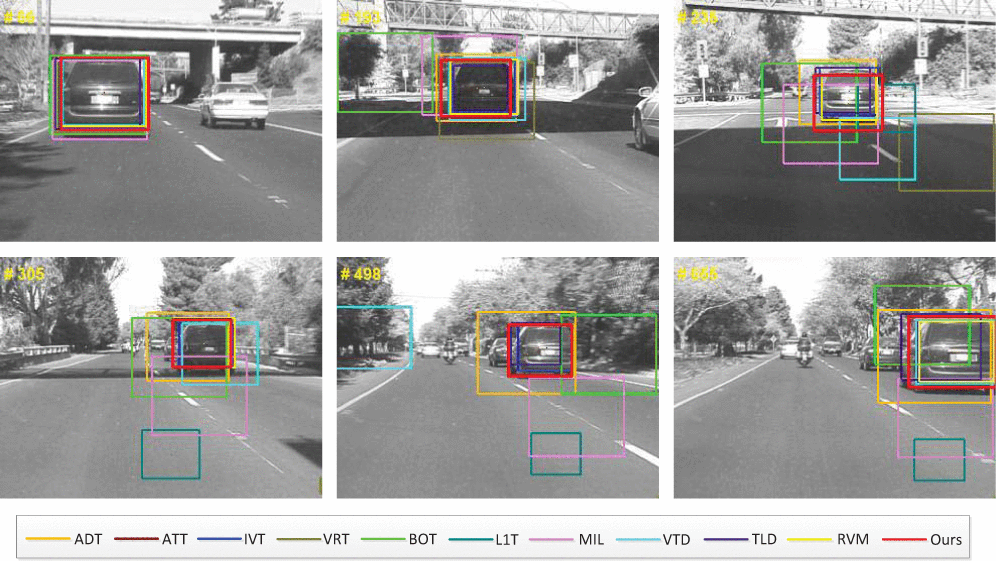
\includegraphics[width=1\textwidth]{tracking}
\caption{Frames from a tracking sequence featuring the bounding boxes indicating results
         of several tracking algorithms. Some examples of drift from the target and
         complete tracking failure can also be observed from some of the boxes.
         Source: Wang et.~al.~fig. 6~\cite{OBJECT_PLS}}\label{fig:tracking}
\end{figure}

\subsection{Target representation}
Early influential works in the field have used target models including subspaces
~\cite{EIGENTRACK} and representing the target as a curve~\cite{CONDENSATION}. Modern
tracking methods can be roughly divided to generative and discriminative, but combinations
of them have also been proposed.~\cite{DLT}

Generative methods search the frame for the best matches to a template of an appearance
model of the subject. Template methods based on pixel intensity and color histograms
perform well with no drastic changes in object appearance and non-cluttered backgrounds.
Appearance models learned from training can be less affected by appearance variations
and adaptive schemes provide added flexibility, while sparse models handle occlusion
and image noise better.~\cite{OBJECT_PLS}

Discriminative methods consider tracking as a binary classification problem. They take
the background also into account to separate the target from it. Used approaches
include refining the initial guess with a support vector machine~\cite{SVT} or utilizing
a relevance vector machine~\cite{SPARSE_BAYESIAN}.

During tracking, the appearance of the target may change for example due to changes in
orientation. Some trackers adapt the tracking model online to be robust against such
changes, but care must be taken in designing the update algorithm as it could result
to drift. Models using online updates have implemented it for example with results of
previous successful tracking results~\cite{BLUR_TRACK}.

\subsection{Datasets}
Research on networks working with image data has been made easier by larger sets of both
hand-labeled data and ones obtained by simple keyword searches from online image services.
With the adoption of unsupervised training and architectures not working as classifiers
unlabeled data can also be used to increase the size of the available training set.
The labeled resources introduced here consist of sets labeled with object classes contained
in the images and ones for tracking with the target marked in each frame.

VOC was a yearly competition for object recognition and VOC 2012 \cite{VOC12} is the last
challenge in the series. The datasets of the challenges are still used for pre-training
features for detection stages in tracking networks. There are four major subsets of
hand-labeled VOC data: classification, segmentation action classification, person layout.
Classification datasets consist of images annotated with the objects contained and bounding
boxes for the objects drawn in the image itself while image segmentation sets provide
additional mask images of the objects and classes in each shot. Action classification sets
contain descriptions and bounding boxes of actions the subjects are performing and person
layout sets contain bounding boxes for the subject's head, hands and feet.
\authorcomment{image examples of the datasets, descriptions to annotations}

The \ac{ilsvrc}~\cite{ILSVRC15} is another recognition challenge running since 2010. The
most recent dataset consists of subsets of object localization, object detection and
object detection from video. The last subset is especially beneficial object tracking
tasks as it provides data for training on actual tracking data. The other two sets are also
substantially larger than the respective VOC sets as their labeling has been crowd sourced.

There has also been an increase in resources solely devoted to tracking data with the
TB-100 -set~\cite{VTB} being a good example. It contains a hundred tracking sequences
with reference positions for the target on each frame. Because some of the targets are
similar or less challenging, a subset of 50 sequences considered challenging is also
provided as TB-50.~\cite{OT_BENCH}

The datasets used for the \ac{vot}~\cite{VOT} can also be used for training networks. The competition
is run yearly with updated evaluation sets which can be used for training as training
data for a network but the challenge itself prohibits training on tracking datasets for
participants.

There is also the yearly \ac{mot}~\cite{MOT16} for testing multiple object trackers but
its unique sequences can also be used to train single object trackers one object at a
time.

\subsection{Evaluation}
Evaluation of proposed trackers is a vital part of the research. It also limits the use
of annotated tracking sequences in training as training and evaluation should be done
on different data.
The Visual Tracker Benchmark~\cite{VTB} is a commonly used resource for comparing
performance to other trackers. It consists of the TB-datasets, a code library containing
implementations of 31 publicly available trackers and ready benchmark results for the
included trackers. The code library is implemented using MATLAB and all included trackers
have been modified to use unified input and output formats. A Python-based testing suite
is also in development. The original benchmark was compiled in 2015 so doesn't include
more recent trackers in the suite. The \ac{vot}~\cite{VOT} and \ac{mot}~\cite{MOT16}
challenges also publish both the yearly challenge suite and results that can used to
compare new networks against the participants.

Precision and success plots are common metrics for comparing trackers against others.
Precision plot is the average center location error over the tracking sequence. This
error is calculated as the distance between the centers of the tracking location and
the hand-labeled ground truth. Success plot represents the average amount of overlap
and the bounding box to the ground truth in relation to their sizes. The overlap score
for a single frame is defined as the union of the boxes divided by their intersection.~\cite{OT_BENCH}
The raw errors can also be used in calculating other indicators. Used examples of these
are precision as the percentage of frames with a center distance error below a set value
and success rate as the percentage of frames with an overlap score above some threshold~\cite{DEEPTRACK}.

\section{Challenges}

Subsections dealing with the present challenges in object tracking and examples for
dealing with them.

\section{Conclusions}

Summarize the current state of object tracking with \ac{dnn}s with possibly some
insight to future developments.


\clearpage
%% Lähdeluettelo

\thesisbibliography{}
\bibliography{kandi}

\begin{appendices}

\begin{otherlanguage}{finnish}
	\clearpage
\section*{Yhteenveto}
Kohteenseuranta videossa on aktiivisesti tutkittu konenäön osa-alue, jossa tavoitteena
on seurata osoitettua kohdetta videossa. Seurantaa ei tule sekoittaa monista älypuhelimistakin
löytyvään tunnistukseen, jossa tarkoitus on vain löytää tietyn kohdeluokan edustajat
kuvasta. Sovelluksia koohteenseurannalla muun muassa videovalvonnassa, koneen ja ihmisen
välisessä viestinnässä sekä lisätyssä todellisuudessa. Luonteeltaan kohteenseurannalla on
yhtäläisyyksiä kuva-analyysisovelluksiin ja myös käytetyt menetelmät ovat osittain samoja.
Viime vuosina kohteenseurantaan onkin sovellettu myös syviä neuroverkkoja niiden menestyttyä
kuvaluokittelussa. Tämän työ perehtyy syväoppimiseen, kohteenseurantaan sekä siihen
käytettyihin syviin neuroverkkoihin. Lisäksi työssä käsitellään tehtävään tarkoitettujen
verkkojen vertailuperiaatteita ja käytettyjä aineistoja. Keskeisimmät tutkimuskysymykset
ovat seuraavat: millaisia syviä neuroverkkorakenteita on käytetty kohteenseurantaan, kuinka
syvien verkkojen käyttö auttaa kyseisissä verkoissa ja mitä heikkouksia syvillä rakenteilla
on seurannan kannalta. Työ on luonteeltaan puhdas kirjallisuuskatsaus.

Keinotekoinen neuroverkko on löyhästi aivojen toimintaperiaatteiden mukaan rakennettu
koneoppimismalli, joka mallinnetaan yleisimmin syötteinä, tulosteina ja niitä yhdistävänä
sarjana kerroksia. Kerrokset koostuvat neuroneista, joilla on sarja painotettuja syötteitä,
syötteiden summalla syötettävä aktivaatiofunktio ja mahdollinen poikkeutusarvo. Kohteenseurannassa
tyypillinen neuronityyppi on tasasuunnattu lineaariyksikkö (rectified linear unit), joka
toteuttaa aktivaatiofunktiota $g (z) = \max\{0,z\}$. Se tuottaa hyöydyllisen epälineaarisen
muunnoksen syötteistä, mutta sen yleistyminen ja optimoinnin keveys ovat silti vertailukelpoisia
lineaaristen mallien kanssa. Syötteet ja tulosteet voidaan mallintaa vektoreina ja painot sekä
poikkeutukset matriiseina.

Syvä neuroverkko tarkoittaa tyypillisesti neuroverkkoa, jossa välikerroksina on monta
piilotettua kerrosta. Koko verkkoa siis opetetaan tuottamaan syötteistä haluttu tuloste
välittämättä yksittäisen välikerroksen tulosteista. Yleisin kohteenseurannassa käytetty
verkkotyyppi on eteenpäin syöttävä eli niin sanottu monikerrosperseptroni (multilayer
perceptron). Eteenpäin syöttävässä verkossa tieto kulkee aina kerroksesta seuraavaan,
eikä niiden välillä ole esimerkiksi takaisinkytkentöjä.

Verkon painot alustetaan tyypillisesti pienillä satunnaisluvuilla ja poikkeutusarvot nollaan
tai pieniin satunnaislukuihin. Yksinkertaisimmillaan koneoppiminen toteutetaan syöttämällä
verkolle tunnettua dataa ja optimoimalla sen painoja vertaamalla tulostetta haluttuun arvoon.
Tulosteen eroa haluttuun arvoon mallinnetaan tappiofunktiolla, jonka gradientti lasketaan
koko verkolle esimerkiksi taaksepäin syöttämällä. Menetelmässä virhearvo syötetään takaisin
pitkin kerroksia ja jokaiselle neuronille asetetaan kontribuutioarvo. Tätä arvoa käytetään
gradientin määrittämiseksi painoille ja kutakin painoa siirretään hieman vastakkaiseen suuntaan
tappiofunktion minimoimiseksi. Prosessia toistetaan uusilla koulutusaineistoilla, kunnes
koulutuksen katsotaan olevan valmis.

Konvoluutiota suoran matriisikertolaskun sijaan vähintään yhdessä kerroksessaan käyttävää
neuroverkkoa kutsutaan konvoluutioneuroverkoksi. Konvoluutio on kahdelle funktiolle suoritettava
operaatio, joka kuvataan yleisesti niiden pistetulojen integraalina toisen funktion
siirtämisen funktiona. Kuva-analyysissä konvoluutio tapahtuu käsittelemällä syötekuvaa
siirrettävällä kernelillä eli matriisilla painoarvoja. Kukin neuroni käsittelee vain
kernelinsä rajoittamaa osaa syötteestä, mutta konvoluutiokerrosten ketjuttamisen myötä
syvemmät kerrokset ovat epäsuorassa yhteydessä koko verkon syötteeseen tai suurimpaan
osaan siitä.

Konvoluutioverkon kerros muodostuu kolmesta vaiheesta: konvoluutiosta, tunnistusksesta ja
keräämisestä. Ne voidaan mallintaa verkkoon erillisinä kerroksina, mikä mahdollistaa
modulaarisen rakenteen. Konvoluutiovaiheessa syöte käsitellään kerneliä liikuttaen.
Tunnistusvaiheessa suoritetaan useita konvoluutioita rinnakkain ja kukin niistä syötetään
lineaariseen aktivaatiofunktioon. Nämä tulosteet syötetään tunnistusvaiheessa epälineaariseen
aktivaatiofunktioon ja keräämisvaiheessa lähekkäiset tunnistuksen tulosteet yhdistetään
keräysfunktiolla.

Kohteenseurantaa videossa on tutkittu vuosikymmeniä. Tyypillisesti seuranta tapahtuu videosta,
jonka ensimmäisessä kuvassa on osoitettu haluttu seurannan kohde, mutta joissain tapauksissa
sovelluksen on löydettävä se kuvauksen perusteella. Tehtävää ei olla laajasta tutkimuksesta
huolimatta ratkaistu, ja seurannan epäonnistumista aiheuttavat edelleen hankalat olosuhteet,
kuten liikeepäterävyys tai kohteen hetkellinen poistuminen kuvasta.

Merkittävät varhaiset sovellukset hyödynsivät kohteesta otettuja kuvasarjoja kohteen etsimiseksi
tai esittivät kohteen sen rajat määrittävänä käyränä. Modernit seurantamenetelmät voidaan jakaa
karkeasti generatiivisiin ja erotteleviin, mutta niiden yhdistelmiä on myös tutkittu. Generatiiviset
sovellukset etsivät kuvasta parhaiten kohteesta muodostettua mallia vastaavia alueita ja erottelevat
toteuttavat seurannan erottamalla kohteen taustasta esimerkiksi soveltamalla luokitteluverkkoa
pienempiin osiin kuvasta.

Koulutukseen käytetyt aineistot ovat yhtä tärkeitä kuin itse verkon rakenne. Seurantaverkkoa
kehitettäessä on tavallista esikouluttaa ominaisuuksia erottelevat kerrokset yksi kerrallaan
esimerkiksi luokitteluun tarkoitettujen käsin merkittyjen tai hakusanalla kuvapalveluista
ladattujen kuva-aineistojen avulla parempien tulosten takaamiseksi. Yksi merkittävimmistä
käytetyistä aineistoista on vuosittaisiin ImageNet Large Scale Visual Recognition Challenge
-haasteisiin päivitettävä kuvakanta.

Yksittäisten kuvien lisäksi koulutukseen käytetään kohteenseurantaan keskittyneitä
videoaineistoja, joilla voidaan arvioida verkon ehdottamaa kohteen sijaintia todelliseen.
Merkittäviä seurantavideoita sisältäviä aineistoja ovat TB-100 ja sen alajoukko TB-50 sekä
vuoteen 2012 järjestetyn Visual Object Tracking challenge (VOT) -kilpailun aineistot.

Kehitettyjä seurantasovelluksia arvioidaan vertaamalla niiden tuloksia aiemmin julkaistuihin
samaa aineistoa käyttämällä. Yksi käytetyistä aineistoista on Visual Tracker Benchmarkin kokoama
TB-50, johon on julkaistu sen tekohetkellä merkittävien vapaasti saatavilla olleiden sovellusten
tulokset vertailua varten. Myös VOT:n kaltaisten kilpailujen tuloksia ja aineistoja voidaan
käyttää myöhempien menetelmien arviointiin.

Viimeaikaiset syviä neuroverkkoja hyödyntävät kohteenseurantasovellukset käyttävät
tyypillisesti konvoluutioneuroverkkoa piirteiden etsimiseen kuvasta, jolloin varsinainen
paikannus voidaan toteuttaa esimerkiksi binäärisenä luokitteluna kohteen ja taustan
välillä. Tavanomaiset käsin määritettyjä malleja käyttävät menetelmät kykenevät seurantaan
hyvin, mikäli videossa ei esiinny hankalia olosuhteita. Syvien verkkojen koulutuksessa
oppimien yleisten piirteiden toivotaan poistavan luokkakohtaisen tiedon tarve menetelmää
suunniteltaessa, sillä yleisten piirteiden avulla verkko voi luoda kohteesta mallin
tuntematta sitä ennakkoon. Verkon painoja voidaan myös säätää seurannan aikana automaattisesti,
mikäli kohteen ulkonäössä havaitaan merkittävä muutos.

Tuoreessa tutkimuksessa on kiinnitetty huomiota syvässä verkossa esiintyvien piirteiden
erilaisiin ominaisuuksiin käsiteltävän tason sijainnista riippuen. Loppupään tasot
tuottavat korkean piirteitä, joista on erityisesti hyötyä kohteen luokittelussa. Aiemmilta
tasoilta voidaan saada tietoa esimerkiksi kohteen tekstuurista tai muista yksilöllisistä
ominaisuuksista, jotka ovat hyödyllisiä seurattavan kohteen erottamisessa mahdollisista
muista samankaltaisista kappaleista. Eritasoisia piirteitä voidaan hyödyntää esimerkiksi
haarauttamalla verkko yhteisiä piirteitä eristävien tasojen jälkeen ja käyttämällä
jalostettuja piirrekarttoja lopulliseen paikallistamiseen seurannan tilasta riippuen.

Julkaistun tutkimuksen perusteella syviä neuroverkkoja hyödyntämällä voidaan kehittää
kilpailukykyisiä kohteenseurantasovelluksia ja esimerkiksi DeepTrackin osoitettiin
kykenevän muita julkaisuhetkellä hallinneita seuraimia parempiin tuloksiin. Syviä
verkkoja on kuitenkin sovellettu kohteenseurantaan vasta verrattain lyhyen ajan, eikä
vertailuja niiden sovellusten välillä ole juurikaan tehty. On siis vaikea tehdä johtopäätöksiä
yksittäisten syvien seurainten paremmuudesta. Suurimpana haasteena on tällä hetkellä
menetelmien huomattavan suuret tehovaatimukset, sillä moni niistä kykeni vain muutaman
kuvan käsittelyyn sekunnissa. Harva toteutus on kuitenkaan ollut erityisesti optimoitu,
joten etenkin saatavilla olevan laskentatehon kasvaessa yhä useammilla menetelmillä voidaan
saavuttaa myös reaaliaikaiseen seurantaan tarvittava käsittelynopeus.

\renewcommand{\thesubsection}{\oldsubection}

\end{otherlanguage}

\end{appendices}

\end{document}
